\documentclass[german,10pt]{book}      
\usepackage{makeidx}
\usepackage{babel}            % Sprachunterstuetzung
\usepackage{amsmath}          % AMS "Grundpaket"
\usepackage{amssymb,amsfonts,amsthm,amscd} 
\usepackage{mathrsfs}
\usepackage{rotating}
\usepackage{sidecap}
\usepackage{graphicx}
\usepackage{color}
\usepackage{fancybox}
\usepackage{tikz}
\usetikzlibrary{arrows,snakes,backgrounds}
\usepackage{hyperref}
\hypersetup{colorlinks=true,
                    linkcolor=blue,
                    filecolor=magenta,
                    urlcolor=cyan,
                    pdftitle={Overleaf Example},
                    pdfpagemode=FullScreen,}
%\newcommand{\hyperref}[1]{\ref{#1}}
%
\definecolor{Gray}{gray}{0.80}
\DeclareMathSymbol{,}{\mathord}{letters}{"3B}
%
\newcounter{num}
\renewcommand{\thenum}{\arabic{num}}
\newenvironment{anmerkungen}
   {\begin{list}{(\thenum)}{%
   \usecounter{num}%
   \leftmargin0pt
   \itemindent5pt
   \topsep0pt
   \labelwidth0pt}%
   }{\end{list}}
%
\renewcommand{\arraystretch}{1.15}                % in Formeln und Tabellen   
\renewcommand{\baselinestretch}{1.15}                 % 1.15 facher
                                                      % Zeilenabst.
\newcommand{\Anmerkung}[1]{{\begin{footnotesize}#1 \end{footnotesize}}\\[0.2cm]}
\newcommand{\comment}[1]{}
\setlength{\parindent}{0em}           % Nicht einruecken am Anfang der Zeile 

\setlength{\textwidth}{15.4cm}
\setlength{\textheight}{23.0cm}
\setlength{\oddsidemargin}{1.0mm} 
\setlength{\evensidemargin}{-6.5mm}
\setlength{\topmargin}{-10mm} 
\setlength{\headheight}{0mm}
\newcommand{\identity}{{\bf 1}}
%
\newcommand{\vs}{\vspace{0.3cm}}
\newcommand{\noi}{\noindent}
\newcommand{\leer}{}

\newcommand{\engl}[1]{[\textit{#1}]}
\parindent 1.2cm
\sloppy

         \begin{document}  \setcounter{chapter}{10}


\chapter{Hebelgesetze --\\von Archimedes bis Mach}
% Kap 11
\label{chap_Hebel}

\info{Thomas Filk}{12.05.2024}%Bildungsplan BW 2022: 3.2.7 (9) (Klasse 7/8)}%
Kaum ein Gesetz bzw.\ eine Gruppe von Gesetzen erscheint zun\"achst\index{Hebel|(}
selbstverst\"andlicher als das Hebelgesetz: Kraft $\times$ Kraftarm = Last $\times$ Lastarm.
In Form einer Gleichgewichtsbedingung f\"ur eine allgemeine Waage kann man\index{Hebelgesetz}\index{Waage}
es auch in der Form \glqq ${\rm Gewicht_1\times Hebelarm}_1= {\rm Gewicht_2\times Hebelarm}_2$\grqq\
formulieren (siehe Abb.\ \ref{fig_Hebel1}).

\begin{figure}[htb]
\begin{picture}(200,120)(0,0)
\put(10,78){\line(1,0){160}}
\put(10,82){\line(1,0){160}}
\put(10,78){\line(0,1){4}}
\put(170,78){\line(0,1){4}}
\put(170,30){\line(0,1){48}}
%
\put(160,30){\line(1,0){20}}
\put(160,10){\line(1,0){20}}
\put(160,10){\line(0,1){20}}
\put(180,10){\line(0,1){20}}
%
\put(100,58){\line(1,0){20}}
\put(100,58){\line(1,2){10}}
\put(120,58){\line(-1,2){10}}
%
\put(10,82){\line(1,1){10}}
\put(10,82){\line(-1,1){10}}
\put(0,92){\line(1,0){5}}
\put(15,92){\line(1,0){5}}
\put(5,92){\line(0,1){20}}
\put(15,92){\line(0,1){20}}
\put(5,112){\line(1,0){10}}
%
\put(10,47){\line(0,1){6}}
\put(10,50){\line(1,0){40}}
\put(70,50){\line(1,0){40}}
\put(110,47){\line(0,1){6}}
\put(60,50){\makebox(0,0){$l_F$}}
\put(110,50){\line(1,0){20}}
\put(150,50){\line(1,0){20}}
\put(140,50){\makebox(0,0){$l_L$}}
\put(10,100){\makebox(0,0){$F$}}
\put(170,20){\makebox(0,0){$L$}}
\end{picture}
\hfill
%%%%
\begin{picture}(200,120)(0,0)
\put(10,78){\line(1,0){160}}
\put(10,82){\line(1,0){160}}
\put(10,78){\line(0,1){4}}
\put(170,78){\line(0,1){4}}
\put(170,30){\line(0,1){48}}
\put(10,30){\line(0,1){48}}
%
\put(160,30){\line(1,0){20}}
\put(160,10){\line(1,0){20}}
\put(160,10){\line(0,1){20}}
\put(180,10){\line(0,1){20}}
%
\put(100,58){\line(1,0){20}}
\put(100,58){\line(1,2){10}}
\put(120,58){\line(-1,2){10}}
%
\put(2,30){\line(1,0){16}}
\put(2,14){\line(1,0){16}}
\put(2,14){\line(0,1){16}}
\put(18,14){\line(0,1){16}}
%
\put(10,47){\line(0,1){6}}
\put(10,50){\line(1,0){40}}
\put(70,50){\line(1,0){40}}
\put(110,47){\line(0,1){6}}
\put(60,50){\makebox(0,0){$l_1$}}
\put(110,50){\line(1,0){20}}
\put(150,50){\line(1,0){20}}
\put(140,50){\makebox(0,0){$l_2$}}
\put(10,21){\makebox(0,0){$G_1$}}
\put(170,20){\makebox(0,0){$G_2$}}
\end{picture}
\caption{\label{fig_Hebel1}%
Zwei Versionen des Hebelgesetzes: (links) Das Produkt aus Kraft ($F$) und Kraftarm ($l_F$) muss
im Gleichgewicht gleich dem Produkt aus Last ($L$) und Lastarm ($l_L$) sein; (rechts) bei einer
Waage ist das Produkt aus den Gewichten ($G_i$) multipliziert mit den zugeh\"origen Hebelarmen 
($l_i$) bei der Gleichgewichtsbedingung auf beiden Seiten gleich.}
\end{figure}
 
Obwohl dieses Gesetz an sich schon sehr einfach ist, kann man dar\"uber diskutieren, ob 
es sich auf einen noch einfacheren
Fall zur\"uckf\"uhren l\"asst. So gibt es \glqq Beweise\grqq\ von Archimedes, Galileo, Huygens und
anderen, bei denen der allgemeine Fall des Hebelgesetzes auf den speziellen symmetrischen
Fall -- Lastarm = Kraftarm und Last = Kraft -- zur\"uckgef\"uhrt wird. Der symmetrische Fall ist
unmittelbar einsichtig und kann als Folge des \glqq Prinzips vom hinreichenden Grund\grqq\ angesehen
werden: Wenn die beiden Hebelarme\index{Prinzip vom hinreichenden Grund}\index{Hebel!symmetrischer Fall}
gleich sind und die beiden Gewichte ebenfalls gleich sind, gibt es keinen Grund, weshalb das
Gleichgewicht zugunsten einer der beiden Seiten gest\"ort sein sollte. Weshalb zu der einen
Seite und nicht zu der anderen? 

Ernst Mach\index{Mach, Ernst} 
argumentiert ganz allgemein gegen die M\"oglichkeit einer solchen Zur\"uckf\"uhrung
des allgemeinen Hebelgesetzes auf den symmetrischen Fall: Falls das allgemeine Hebelgesetz
von der Form $G_1 f(l_1) = G_2 f(l_2)$ w\"are, mit einer beliebigen Funktion $f$ (z.B.\ k\"onnte
gelten $f(l)=l^p$), w\"urde trotzdem der symmetrische Fall gelten, d.h.\ das Gesetz w\"are f\"ur
$G_1=G_2$ und $l_1=l_2$ erf\"ullt. Insofern kann es nach Mach nicht m\"oglich sein, das
allgemeine Hebelgesetz aus seiner symmetrischen Form abzuleiten. 

Trotzdem ist es interessant zu untersuchen, an welchen Stellen Archimedes und seine Nachfolger
weitere, teilweise versteckte Annahmen hineinstecken, wenn sie glauben, das allgemeine Gesetz 
aus dem speziellen ableiten
zu k\"onnen. W\"ahrend Ernst Mach argumentiert, dass die allgemeine Form des Hebelgesetzes
in versteckter Form bei diesen Beweisen verwendet wird, erscheinen mir andere Annahmen gemacht
zu werden, die dann zwar das Hebelgesetz zur Folge haben, aber physikalisch begr\"undeter sind. 
Die folgenden Darstellungen lehnen sich eng an die Untersuchung von Ernst Mach
an \cite{Mach}.

\section{Der Beweis von Archimedes}

Archimedes (um 287--212\,v.Chr.)\index{Archimedes} 
geht von einer zus\"atzlichen Erfahrungstatsache aus: Eine symmetrische Waage mit zwei
gleichen Gewichten $G$ und gleichen Hebelarmen steht im Gleichgewicht mit einem Gewicht
zu der doppelten Masse, also $2G$ (siehe Abb.\ \ref{fig_Hebel2}). 

\begin{SCfigure}[50][htb]
\begin{picture}(200,120)(0,0)
\put(20,58){\line(1,0){100}}
\put(20,62){\line(1,0){100}}
\put(20,58){\line(0,1){4}}
\put(120,58){\line(0,1){4}}
%
\put(120,30){\line(0,1){28}}
\put(110,30){\line(1,0){20}}
\put(110,10){\line(1,0){20}}
\put(110,10){\line(0,1){20}}
\put(130,10){\line(0,1){20}}
%
\put(20,30){\line(0,1){28}}
\put(10,30){\line(1,0){20}}
\put(10,10){\line(1,0){20}}
\put(10,10){\line(0,1){20}}
\put(30,10){\line(0,1){20}}
%
\put(80,100){\circle{20}}
\put(80,100){\makebox(0,0){$\bullet$}}
\put(160,100){\makebox(0,0){$\bullet$}}
\put(70,62){\line(0,1){38}}
\put(80,110){\line(1,0){80}}
\put(160,100){\circle{20}}
\put(170,33){\line(0,1){67}}
%
\put(157,33){\line(1,0){26}}
\put(157,7){\line(1,0){26}}
\put(157,7){\line(0,1){26}}
\put(183,7){\line(0,1){26}}
\put(170,20){\makebox(0,0){$2G$}}
\put(120,20){\makebox(0,0){$G$}}
\put(20,20){\makebox(0,0){$G$}}
\put(70,62){\makebox(0,0){$\bullet$}}
\end{picture}
\caption{\label{fig_Hebel2}%
Eine symmetrische Waage mit zwei Gewichten $G$ kann in der Mitte durch ein einzelnes,
doppelt so gro\ss es Gewicht $2G$ ersetzt werden. Hier (und im Folgenden) wird angenommen, dass
die Masse des Hebelarms im Vergleich zu den Massen $m$ zu den Gewichten $G=mg$, $g$ die
Schwerbeschleunigung auf der Erdoberfl\"ache, vernachl\"assigt werden kann.}
\end{SCfigure}

Diese\index{Archimedes!Beweis des Hebelgesetzes} 
Beobachtung wendet Archimedes auf eine symmetrische Situation an, bei der
eine Waage mit drei gleichen Gewichten $G$ gegeben ist, von denen zwei am 
\"au\ss eren Rand und eines in der Mitte angebracht ist (siehe Abb.\ \ref{fig_Hebel3}, links). 
Diese Situation ist symmetrisch und sollte im Gleichgewicht sein. Nun wendet er
die obige Ersetzung von zwei Gewichten durch ein einzelnes, doppelt so schweres
Gewicht auf die beiden Gewichte an, die sich an der linken Seite bzw.\ in der Mitte
befinden (Abb.\ \ref{fig_Hebel3}, rechts). Er gelangt so zu einem einfachen asymmetrischen
Fall, bei dem sich auf der einen Seite das Gewicht $2G$, auf der anderen Seite das
Gewicht $G$ befindet, und die beiden Hebelarme das Verh\"altnis 1:2 haben. 

\begin{figure}[htb]
\begin{picture}(200,90)(0,0)
\put(20,58){\line(1,0){160}}
\put(20,62){\line(1,0){160}}
\put(20,58){\line(0,1){4}}
\put(180,58){\line(0,1){4}}
\put(100,62){\line(0,1){25}}
%
\put(180,30){\line(0,1){28}}
\put(170,30){\line(1,0){20}}
\put(170,10){\line(1,0){20}}
\put(170,10){\line(0,1){20}}
\put(190,10){\line(0,1){20}}
%
\put(20,30){\line(0,1){28}}
\put(10,30){\line(1,0){20}}
\put(10,10){\line(1,0){20}}
\put(10,10){\line(0,1){20}}
\put(30,10){\line(0,1){20}}
%
\put(100,30){\line(0,1){28}}
\put(90,30){\line(1,0){20}}
\put(90,10){\line(1,0){20}}
\put(90,10){\line(0,1){20}}
\put(110,10){\line(0,1){20}}
%
\put(20,50){\line(1,0){35}}
\put(65,50){\line(1,0){35}}
\put(60,50){\makebox(0,0){$l$}}
\put(100,50){\line(1,0){35}}
\put(145,50){\line(1,0){35}}
\put(140,50){\makebox(0,0){$l$}}
%
\put(180,20){\makebox(0,0){$G$}}
\put(100,20){\makebox(0,0){$G$}}
\put(20,20){\makebox(0,0){$G$}}
\put(100,62){\makebox(0,0){$\bullet$}}
\end{picture}
\hfill
%%%%
\begin{picture}(200,90)(0,0)
\put(20,58){\line(1,0){160}}
\put(20,62){\line(1,0){160}}
\put(20,58){\line(0,1){4}}
\put(180,58){\line(0,1){4}}
\put(100,62){\line(0,1){25}}
%
\put(180,30){\line(0,1){28}}
\put(170,30){\line(1,0){20}}
\put(170,10){\line(1,0){20}}
\put(170,10){\line(0,1){20}}
\put(190,10){\line(0,1){20}}
%
\put(60,33){\line(0,1){25}}
\put(47,33){\line(1,0){26}}
\put(47,7){\line(1,0){26}}
\put(47,7){\line(0,1){26}}
\put(73,7){\line(0,1){26}}
%
%\put(10,47){\line(0,1){6}}
\put(60,50){\line(1,0){15}}
\put(85,50){\line(1,0){15}}
\put(100,47){\line(0,1){6}}
\put(80,50){\makebox(0,0){$\frac{l}{2}$}}
\put(100,50){\line(1,0){35}}
\put(145,50){\line(1,0){35}}
\put(140,50){\makebox(0,0){$l$}}
%
\put(180,20){\makebox(0,0){$G$}}
\put(60,20){\makebox(0,0){$2G$}}
\put(100,62){\makebox(0,0){$\bullet$}}
\end{picture}
\caption{\label{fig_Hebel3}%
Werden bei dem symmetrischen Fall (links), bei dem die Waage 
im Gleichgewicht sein sollte, die beiden linken Gewichte durch ein doppelt
so gro\ss es Gewicht in der Mitte ersetzt, erhalten wir ein einfaches Beispiel
f\"ur den asymmetrischen Fall. Das Verh\"altnis der Gewichte ist 2:1, das der
zugeh\"origen Hebelarme 1:2.}
\end{figure}

Man kann sich nun leicht symmetrische Situationen vorstellen, bei denen mehr als
drei Gewichte im Gleichgewicht sind und die man durch eine entsprechende
Ersetzung in den allgemeinen Hebelfall \"ubertragen kann. Dies wird bei den
Herleitungen von Galileo und Stevin verwendet und dort nochmals aufgegriffen
(siehe Abschnitt \ref{sec_Hebel_G}). Auf eine allgemeine Diskussion der Annahmen,
die Archimedes in seinen \glqq Beweis\grqq\ hat einflie\ss en lassen, kommen wir
anschlie\ss end zu sprechen.

\section{Die Ableitung von Galileo und Stevin}
\label{sec_Hebel_G}

Galileo Galilei (1564--1641)\index{Galilei, Galileo}\index{Stevin, Simon} 
und Simon Stevin (1548/49--1620) leiteten das
Hebelgesetz aus einer \"ahnlichen Annahme wie Archimedes ab. Sie gehen
davon aus, dass eine Massenverteilung einen Schwerpunkt hat, um den man
die Massenverteilung auch beliebig drehen kann (siehe Abb.\ \ref{fig_Mach}). 

\begin{SCfigure}[50][htb]
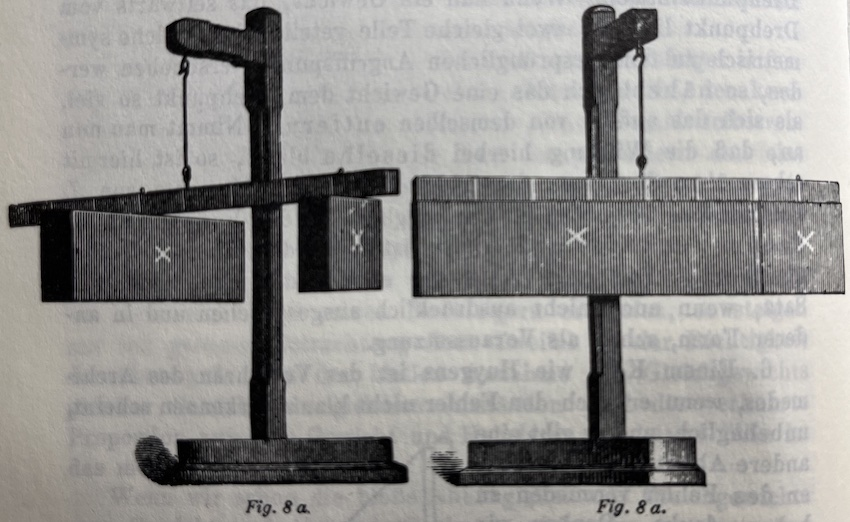
\includegraphics[width=0.6\textwidth]{./Bilder/Mach.jpg}
\caption{\label{fig_Mach}%
Die Beweise von Galileo und Stevin setzen die Existenz eines Schwerpunkts voraus,
der sich nicht \"andert, wenn man die Massenverteilung um diesen Schwerpunkt
dreht. Im Bild wurde der symmetrische Fall (rechts) in zwei Teile aufgeteilt, die dann um 
ihren jeweiligen Schwerpunkt gedreht wurden (links). Man gelangt so zu einem asymmetrischen
Fall. (aus \cite{Mach})}
\end{SCfigure}

Es handelt sich hierbei um eine Verallgemeinerung des Beweises von Archimedes
auf eine kontinuierliche Massenverteilung. Gegeben sei der symmetrische Fall
einer Waage, bei der eine homogene Massenverteilung entlang einer Scheibe
in der Mitte an einem Faden aufgeh\"angt ist. Diese Masse wird in
zwei unterschiedliche Massen aufgeteilt, indem sie senkrecht in zwei Teile
unterteilt wird (Abb.\ \ref{fig_Mach}, rechts). Nun wird f\"ur beide Teile der symmetrische
Fall postuliert, d.h., es gibt in der Mitte beider Teile jeweils einen Aufh\"angepunkt,
um den die Masse gedreht werden kann, ohne dass sich etwas \"andert (Abb.\ \ref{fig_Mach}, links). 
Man erh\"alt so den allgemeinen Fall des Hebelgesetzes. 

\begin{SCfigure}[50][htb]
\begin{picture}(200,100)(0,0)
\put(10,20){\line(1,0){180}}
\put(10,60){\line(1,0){180}}
\put(10,20){\line(0,1){40}}
\put(190,20){\line(0,1){40}}
\put(130,20){\line(0,1){40}}
%
\put(100,60){\line(0,1){30}}
%
\put(100,60){\makebox(0,0){$\bullet$}}
\put(160,60){\makebox(0,0){$\bullet$}}
\put(70,60){\makebox(0,0){$\bullet$}}
%
\put(10,7){\line(0,1){6}}
\put(130,7){\line(0,1){6}}
\put(190,7){\line(0,1){6}}
\put(10,10){\line(1,0){55}}
\put(75,10){\line(1,0){55}}
\put(130,10){\line(1,0){25}}
\put(165,10){\line(1,0){25}}
%
\put(70,72){\line(0,1){6}}
\put(160,72){\line(0,1){6}}
\put(70,75){\line(1,0){10}}
\put(90,75){\line(1,0){10}}
\put(100,75){\line(1,0){25}}
\put(135,75){\line(1,0){25}}
%
\put(70,10){\makebox(0,0){$l_1$}}
\put(160,10){\makebox(0,0){$l_2$}}
\put(85,75){\makebox(0,0){$x_1$}}
\put(130,75){\makebox(0,0){$x_2$}}
\put(70,40){\makebox(0,0){$m_1$}}
\put(160,40){\makebox(0,0){$m_2$}}
\end{picture}
\caption{\label{fig_Hebel4}%
Die symmetrische Aufh\"angung eines homogenen Stabes des Masse $m$ in zwei
Teile der jeweiligen Massen $m_1$ und $m_2$ entspricht auch der Aufteilung der Gesamtl\"ange $l$
in die Anteile $l_1$ und $l_2$ mit $l_1+l_2=l$. Die Hebell\"angen der Schwerpunkte sind
$x_1$ bzw.\ $x_2$.}
\end{SCfigure}

Die gesamte Hebell\"ange ist $l_1+l_2$ und somit hat jeder Hebel die L\"ange
$(l_1+l_2)/2$. Damit ergeben sich aus Abb.\ \ref{fig_Hebel4} f\"ur die neuen Hebelarme
$x_1$ und $x_2$ die folgenden Gleichungen:
\begin{equation}
        x_1 = \frac{l_1+l_2}{2} - \frac{l_1}{2} = \frac{l_2}{2} \hspace{1cm} {\rm und} \hspace{1cm}
        x_2 = \frac{l_1+l_2}{2} - \frac{l_2}{2} = \frac{l_1}{2} \, .
\end{equation}
Die neuen Hebelarme $x_1:x_2$ stehen also in dem Verh\"altnis $l_2:l_1$. Und da die
Massen $m_1$ und $m_2$ in demselben Verh\"altnis wie die L\"angen stehen, ergibt sich insgesamt
$m_1:m_2=l_1:l_2=x_2:x_1$ oder
\begin{equation}
        m_1 \cdot x_1 = m_2 \cdot x_2 \, .
\end{equation}
Wir erhalten somit das allgemeine Hebelgesetz.\index{Hebelgesetz} 

\section{Die Existenz eines Schwerpunkts}

Sowohl Archimedes als auch Galileo und Stevin setzen voraus, dass es zu einer
Massenverteilung einen Punkt gibt, sodass man sich die gesamte Masse in diesem\index{Schwerpunkt}
Punkt vereint denken kann, und dass sich statische Gleichgewichtsverh\"altnisse, wie sie bei 
einer Waage oder einem Hebel vorliegen, dadurch nicht \"andern. Die wesentliche Annahme ist, 
dass dieser Punkt nur von der Verteilung der Massen selbst, nicht aber von der Umgebung
und der Verteilung von Massen in der Umgebung abh\"angt, und dass sich auch an den
Gleichgewichtsverh\"altnissen in der Umgebung nichts \"andert, wenn Massenverteilungen durch 
eine einzelne Masse in ihrem
Schwerpunkt ersetzt werden. In Abb.\ \ref{fig_Hebel2} wird
diese Annahme bei Archimedes deutlich.

Wenn wir somit annehmen, dass es zu einer Massenverteilung einen Schwerpunkt gibt
und dass wir uns die Gesamtmasse als punktf\"ormig in diesem Schwerpunkt 
konzentriert denken d\"urfen, ohne dass sich in der Umgebung etwas \"andert, dann
sind die Argumente von Archimedes, Galileo und Stevin g\"ultig und wir k\"onnen den
allgemeinen Fall des Hebelgesetzes aus dem speziellen symmetrischen Fall ableiten. 

Dass eine solche Annahme nicht selbstverst\"andlich ist, erkennen wir an einer
\"ahnlichen physikalischen Situation, die sich aber auf eine andere Gr\"o\ss e bezieht.
Wenn wir zwei Massen in einem Abstand $2l$ haben, hat dieser K\"orper ein
Tr\"agheitsmoment $M=2ml^2$ (genauer hat dieser K\"orper einen Tr\"agheitstensor,
von dem zwei Haupttr\"agheitsmomente den Wert $M=2ml^2$ haben und ein
Haupttr\"agheitsmoment n\"aherungsweise null ist). 
Wir k\"onnen uns hier die Masse nicht in den Mittelpunkt konzentriert denken und argumentieren, 
dass sich das Tr\"agheitsmoment nicht ge\"andert hat. 

Wir k\"onnen somit die Annahmen, die \"uber den symmetrischen Fall hinausgehen,
folgenderma\ss en zusammenfassen:
\begin{enumerate}
\item
Zu jeder (starren) Massenverteilung gibt es einen Punkt, den Schwerpunkt, sodass eine
Aufh\"angung in diesem Punkt die Massenverteilung im Gleichgewicht l\"asst.
\item
Die Gesamtmasse (Summe aller Einzelmassen der Masseverteilung) steht mit der
vorgegebenen Masseverteilung im Gleichgewicht.
\item
Statt der vorgegebenen Masseverteilung kann man sich die Gesamtmasse im 
Schwerpunkt konzentriert denken, ohne dass sich an den Schwerpunkten einer
allgemeineren Masseverteilung etwas \"andert. Mit anderen Worten: Gibt es eine
Massenverteilung $\{M= m_1 + m_2 +... +m_n\}$ mit einem Schwerpunkt $\vec{S}$, und sei
$\{\hat{m}_1=m_1 +... +m_k\}$ eine Teilmenge von $M$ mit Schwerpunkt $\vec{s}_1$, dann
k\"onnen wir die Gesamtmasse der Teilmenge $\hat{m}_1$ in den Schwerpunkt $\vec{s}_1$ legen,
ohne dass sich an $\vec{S}$ etwas \"andert.
\end{enumerate}
Die letzte Bedingung ist sehr einschr\"ankend und gilt beispielsweise f\"ur
Tr\"agheitsmomente nicht. Die Ersetzung von Massenverteilungen durch eine Gesamtmasse
im Schwerpunkt ist die Bedingung, die das Hebelgesetz als lineare Funktion des Hebelarms
auszeichnet. Der Beweis, dass das \"ubliche Hebelgesetz diese Eigenschaft besitzt, ist sehr einfach,
hier f\"ur die Unterteilung einer Massenverteilung in zwei Teilmengen:
\begin{eqnarray}
    \vec{S} &=& \frac{1}{M}  \left( \sum_{i=1}^n m_i \vec{x}_i \right) 
          = \frac{1}{M}  \left(  \hat{m}_1 \cdot \frac{1}{\hat{m}_1} \sum_{i=1}^k m_i \vec{x}_i +
              \hat{m}_2 \cdot \frac{1}{\hat{m}_2} \sum_{i=k+1}^n m_i \vec{x}_i \right)  \\
          &=&  \frac{1}{\hat{m}_1+\hat{m}_2} \left(  \hat{m}_1 \vec{s}_1 +
              \hat{m}_2  \vec{s}_2 \right)     
\end{eqnarray}
mit
\begin{equation}
      M =   \sum_{i=1}^n m_i \hspace{1cm}  \hat{m}_1= \sum_{i=1}^k m_i  \hspace{1cm}  \hat{m}_2= \sum_{i=k+1}^n m_i \, .
\end{equation}

\section{Der \glqq Beweis\grqq\ von Huygens}

Christiaan Huygens (1629--1695)\index{Huygens, Christiaan} 
betrachtet eine Massenverteilung in der Ebene, die der Massenverteilung bei Galileo
bzw.\ Stevin entspricht, nachdem dort die massiven Balken (Mach spricht immer von Prismen)
gedreht wurden (Abb.\ \ref{fig_Mach}, links), siehe Abb.\ \ref{fig_Hebel_Huygens} (links).  
Die Balken der L\"ange $l_1$ und $l_2$ haben eine konstante Massendichte und ihre
Massen $m_1$ und $m_2$ stehen daher im selben Verh\"altnis wie die L\"angen:
$m_1:m_2=l_1:l_2$. Diese beiden Balken liegen parallel zueinander und senkrecht zu ihrer
Verbindungslinie im Abstand $x$. 

\begin{figure}[htb]
\begin{picture}(190,200)(0,0)
\put(10,10){\line(1,0){5}}
\put(10,10){\line(0,1){180}}
\put(10,190){\line(1,0){5}}
\put(15,10){\line(0,1){180}}
\put(12.5,100){\makebox(0,0){$\bullet$}}
\put(170,70){\line(1,0){5}}
\put(170,70){\line(0,1){60}}
\put(170,130){\line(1,0){5}}
\put(175,70){\line(0,1){60}}
\put(172.5,100){\makebox(0,0){$\bullet$}}
\put(52.5,100){\makebox(0,0){$\bullet$}}
\multiput(10,130)(13,0){13}{\line(1,0){5}}
\multiput(10,10)(13,0){13}{\line(1,0){5}}
\put(3,100){\makebox(0,0){$M$}}
\put(180,100){\makebox(0,0){$N$}}
\put(12.5,100){\line(1,0){160}}
\put(12.5,130){\line(4,-3){160}}
%
\put(52.5,107){\makebox(0,0){$S$}}
\put(3,10){\makebox(0,0){$A$}}
\put(3,190){\makebox(0,0){$B$}}
\put(3,130){\makebox(0,0){$C$}}
\put(178,10){\makebox(0,0){$D$}}
\put(180,70){\makebox(0,0){$E$}}
\put(180,130){\makebox(0,0){$F$}}
\end{picture}
\hfill
%
\begin{picture}(30,200)(0,0)
\put(0,10){\line(1,0){10}}
\put(0,190){\line(1,0){10}}
\put(5,10){\line(0,1){85}}
\put(5,105){\line(0,1){85}}
\put(20,70){\line(1,0){10}}
\put(20,130){\line(1,0){10}}
\put(25,70){\line(0,1){25}}
\put(25,105){\line(0,1){25}}
\put(5,100){\makebox(0,0){$l_1$}}
\put(25,100){\makebox(0,0){$l_2$}}
\end{picture}
\hfill
%
\begin{picture}(190,200)(0,0)
\put(10,10){\line(1,0){5}}
\put(10,10){\line(0,1){120}}
\multiput(10,130)(0,10){6}{\line(0,1){5}}
\multiput(15,130)(0,10){6}{\line(0,1){5}}
\put(10,190){\line(1,0){5}}
\put(15,10){\line(0,1){120}}
\put(12.5,100){\makebox(0,0){$\bullet$}}
\put(170,70){\line(1,0){5}}
\put(170,70){\line(0,1){60}}
\put(170,130){\line(1,0){5}}
\put(175,70){\line(0,1){60}}
\put(172.5,100){\makebox(0,0){$\bullet$}}
\put(52.5,100){\makebox(0,0){$\bullet$}}
\multiput(10,130)(13,0){13}{\line(1,0){5}}
%\multiput(16.5,187)(20,-15){8}{\line(4,-3){10}}
\multiput(12.0,187.5)(4,-3){41}{$\cdot$}
\put(12.5,130){\line(4,-3){160}}
\put(12.5,100){\line(1,0){160}}
\put(3,100){\makebox(0,0){$M$}}
\put(180,100){\makebox(0,0){$N$}}
\put(40,92){\makebox(0,0){$x_1$}}
\put(120,92){\makebox(0,0){$x_2$}}
\put(28,150){\makebox(0,0){$\frac{l_1-l_2}{2}$}}
\put(28,55){\makebox(0,0){$\frac{l_1+l_2}{2}$}}
\put(170,10){\line(1,0){5}}
\put(170,10){\line(0,1){60}}
%\put(170,70){\line(1,0){5}}
\put(175,10){\line(0,1){60}}
\put(52.5,107){\makebox(0,0){$S$}}
\put(3,10){\makebox(0,0){$A$}}
\put(3,190){\makebox(0,0){$B$}}
\put(3,130){\makebox(0,0){$C$}}
\put(178,10){\makebox(0,0){$D$}}
\put(180,70){\makebox(0,0){$E$}}
\put(180,130){\makebox(0,0){$F$}}
\end{picture}
\caption{\label{fig_Hebel_Huygens}%
Der Beweis von Huygens f\"ur das allgemeine Hebelgesetz. (links) Huygens
m\"ochte beweisen, dass eine Masse $m_1$ proportional zu $l_1$ (einem massiven
Stab $AB$ der L\"ange $l_1$) im Gleichgewicht zu einer Masse $m_2$ ist (die durch
einen massiven Stab $EF$ der L\"ange $l_2$ mit derselben L\"angendichte wie Stab 1 
gegeben ist), sofern der Gleichgewichtspunkt $S$ den Abstand der Aufh\"angungen
im Verh\"altnis $x_1:x_2=l_2:l_1$ teilt. Er beweist dazu, dass nicht nur die symmetrische
Linie $MN$ sondern auch die Verbindungslinie
$CD$ eine Symmetrieachse ist. (rechts) Daf\"ur verschiebt er in Gedanken den Teil  
$CB$ des l\"angeren Balkens entlang der Linie $CD$ zu der Lage $DE$. Dies sollte das 
Gleichgewicht um die Achse $CD$ nicht \"andern. Die Massen liegen nun auf
den Teilen $AC$ und $DF$.
Bei der neuen Massenverteilung liegt aber ein symmetrischer
Fall um die Achse $CD$ vor, daher sollte um diese Achse Gleichgewicht herrschen.}
\end{figure}

Huygens argumentiert nun folgenderma\ss en: Wenn es einen Schwerpunkt $S$ gibt, muss
dieser aus Symmetriegr\"unden auf der Verbindungslinie $MN$ der Mittelpunkte liegen. Wenn
die Massenanordnung in ihrem Schwerpunkt im Gleichgewicht ist, muss sie auch auf
jeder Geraden durch den Schwerpunkt im Gleichgewicht sein. Wir k\"onnen die (masselos gedachte)
Ebene mit den beiden massiven Balken somit auf eine scharfe Kante durch den Schwerpunkt legen und
die Anordnung sollte (im Idealfall) zu keiner der beiden Seiten dieser Kante kippen. 
Umgekehrt: Wenn man zwei Kanten findet, f\"ur die die Massenverteilung im Gleichgewicht
ist, kann der Schwerpunkt der Massenverteilung nur der Schnittpunkt dieser beiden Kanten
sein. Huygens behauptet nun, dass die Linie $CD$ in Abb.\ \ref{fig_Hebel_Huygens} ebenfalls
eine Symmetrielinie der Massenanordnung ist, so dass auf einer Kante entlang dieser Linie 
die Anordnung im Gleichgewicht ist. 

Um zu beweisen, dass $CD$ ebenfalls eine Symmetrielinie darstellt, verschiebt Huygens
das Massest\"uck $CB$, um das der l\"angere der beiden Balken \"uber den k\"urzeren
Balken hinausragt, parallel entlang der Linie $CD$ zu dem k\"urzeren Balken in die Position
$DE$ (siehe Abb.\ \ref{fig_Hebel_Huygens}, rechts). Er erh\"alt auf diese Weise zwei Balken gleicher
L\"ange (die Balken $AC$ und $DF$), die jeweils unter gleichem Winkel von der Verbindungslinie 
$CD$ abstehen. Daher ist die Massenverteilung nun symmetrisch zu der Linie $CD$ und 
sollte in Bezug auf diese Linie
im Gleichgewicht sein. Andererseits sollte die Verschiebung einer Masse parallel zu einer Linie, 
sodass sich der Abstand der Masse von dieser Linie nicht \"andert, an den 
Gleichgewichtsverh\"altnissen relativ zu dieser Linie nichts \"andern. 

Da Huygens nun zwei unabh\"angige Linien gefunden hat, um die die Massenverteilung im
Gleichgewicht ist, kann ein m\"oglicher Schwerpunkt nur der Schnittpunkt $S$ dieser Linien sein. 
Dass die Lage dieses Schnittpunkts mit dem \"ublichen Hebelgesetz \"ubereinstimmt, kann man
leicht aus geometrischen \"Uberlegungen ableiten: Die beiden Dreiecke $CMS$ und $DNS$ sind
einander \"ahnlich, sodass sich die beiden Streckenabschnitte $x_1$ und $x_2$ wie die
Abschnitte $MC=l_2/2$ und $ND=l_1/2$ verhalten. Also gilt $x_1:x_2=l_2:l_1$ und damit
auch $x_1:x_2=m_2:m_1$, also das bekannte Hebelgesetz.

Mach behauptet nun, dass das zu Beweisende bei der Schlussfolgerung hineingesteckt wird.
Die Verschiebung gesteht er Huygens zu, da hierbei keine Abst\"ande von einer Gleichgewichtsachse
ver\"andert werden. Er argumentiert aber, dass der Schnittpunkt von
zwei Achsen, um die Gleichgewicht herrscht, nur dann ein Schwerpunkt ist, wenn diese Achsen
senkrecht aufeinander stehen, was im vorliegenden Beispiel nicht der Fall ist. Dazu bestimmt Mach einen
Schwerpunkt bez\"uglich der $x$-Achse eines Koordinatensystems und einen Schwerpunkt 
bez\"uglich der $y$-Achse des Koordinatensystems und zeigt, dass diese beiden so bestimmten
Schwerpunkte nur dann unter einer Drehung des Koordinatensystems invariant sind, wenn das
allgemeine Hebelgesetz gilt. 

Man kann daher auch sagen: Das allgemeine Hebelgesetz folgt aus dem symmetrischen Fall, sofern
angenommen werden darf, dass es einen eindeutigen Schwerpunkt gibt und dass die Lage
dieses Schwerpunkts nicht von der Wahl des Koordinatensystems abh\"angt. Aus der zweiten
Annahme folgt somit, dass auch f\"ur jede Achse durch den Schwerpunkt Gleichgewicht herrscht und
damit ist umgekehrt der Schluss zul\"assig, das der Schwerpunkt der Schnittpunkt von zwei
linear unabh\"angigen Gleichgewichtsachsen sein muss.

Interessant an der Huygens'schen Argumentation ist, dass die L\"ange der Balken keine Rolle
spielt, solange die L\"ange proportional zur Masse ist. Man kann die Balken also sehr kurz machen.
Die Linie $CD$ r\"uckt dann zwar immer mehr an die symmetrische Verbindungslinie $MN$ heran,
aber sie beh\"alt ihren Schnittpunkt mit dieser Linie. 

\section{Der allgemeine schiefwinklige Hebel}

Mach zeigt schlie\ss lich, dass das allgemeine Hebelgesetz, bei dem die Hebelarme nicht
parallel zueinander liegen, aus dem oben angegebenen Hebelgesetz sowie einer
verallgemeinerten Symmetrieannahme folgt.\index{Hebel!schiefwinkliger} 

Zun\"achst betrachtet Mach einen symmetrischen Fall, bei dem die Kr\"afte und die senkrecht zu den
Kr\"aften stehenden Hebelarme gleich sind und bei dem es eine Symmetrieachse bzw.\ Symmetrieebene
gibt (siehe Abb.\ \ref{fig_Hebel_Allg}, links). Diese Situation beschreibt ein Gleichgewicht aus
Symmetriegr\"unden.\index{Hebel!symmetrischer} 
Mach argumentiert weiterhin, dass die kreisf\"ormige Umsetzung der Kr\"afte nur die beiden
senkrechten Hebelarme der L\"ange $l$ ben\"otigt und die Kreisscheibe auf diese reduziert werden kann.

\begin{figure}[htb]
\begin{picture}(170,120)(0,0)
\put(50,70){\circle{40}}
\put(31,74){\vector(-1,-4){15}}
\put(31,74){\makebox(0,0){$\bullet$}}
\put(65,83){\vector(1,-1){50}}
\put(64,84){\makebox(0,0){$\bullet$}}
\put(50,70){\makebox(0,0){$\bullet$}}
\put(50,70){\line(1,1){14}}
\put(50,70){\line(-4,1){18}}
\multiput(40,110)(1,-4){25}{\makebox(0,0){$\cdot$}}
\put(24,20){\makebox(0,0){$F$}}
\put(104,35){\makebox(0,0){$F$}}
\put(40,67){\makebox(0,0){$l$}}
\put(61,74){\makebox(0,0){$l$}}
\end{picture}
%
\begin{tikzpicture}
\draw (20mm,20mm) circle (6mm);
\draw (20mm,20mm) circle (12mm);
\draw [->,thick] (8mm,20mm) -- (8mm,10mm);
\draw [->,thick] (24.5mm,24mm) -- (41mm,6mm);
\draw [thick] (8mm,20mm) -- (20mm,20mm) -- (24.5mm,24mm);
\draw (5mm,15mm) node {$F_1$};
\draw (34mm,10mm) node {$F_2$};
\draw (20mm,20mm) node {$\bullet$};
\draw (12mm,18mm) node {$l_1$};
\draw (23mm,19mm) node {$l_2$};
%
\draw (70mm,20mm) circle (6mm);
\draw (70mm,20mm) circle (12mm);
\draw [->,thick] (58mm,20mm) -- (58mm,10mm);
\draw [->,thick] (74.5mm,24mm) -- (91mm,6mm);
\draw [->,thick] (64mm,20mm) -- (64mm,0mm);
\draw [->,thick] (76mm,20mm) -- (76mm,0mm);
\draw [thick] (58mm,20mm) -- (70mm,20mm) -- (74.5mm,24mm);
\draw (55mm,15mm) node {$F_1$};
\draw (84mm,10mm) node {$F_2$};
\draw (61.5mm,5mm) node {$F_2$};
\draw (78.5mm,5mm) node {$F_2$};
\draw (70mm,20mm) node {$\bullet$};
\draw (62mm,18mm) node {$l_1$};
\draw (73mm,19mm) node {$l_2$};
\draw (55mm,0mm) node {(1)};
\draw (61.5mm,0mm) node {(2)};
\draw (78.5mm,0mm) node {(3)};
\draw (84mm,0mm) node {(4)};
\end{tikzpicture}
\caption{\label{fig_Hebel_Allg}%
(links) Der schiefwinklige symmetrische Fall des Hebelgesetzes. Hier sind die
senkrechten Hebelarme sowie die Kr\"afte gleich. Es gibt eine Symmetrieachse entlang
der gestrichelten Linie. (mitte) Beim allgemeinen schiefwinkligen
Fall sind die Kr\"afte und die senkrechten Hebelarme verschieden, aber das Produkt
von beiden ist gleich. (rechts) Der allgemeine Fall l\"asst sich auf zwei spezielle F\"alle
zur\"uckf\"uhren, indem man um einen symmetrischen Fall erweitert, bei dem zwei Kr\"afte $F_2$
bei (2) und (3)
auf dem kleineren Rad hinzugef\"ugt werden. Diese Situation l\"asst sich auch anders
interpretieren: Die Kr\"afte (2) und (4) sind gleich, ebenso die Hebelarme, sodass diese
beiden den symmetrischen Gleichgewichtsfall (links) darstellen. 
Au\ss erdem bilden die Kr\"afte (1) und (3) sowie die
zugeh\"origen Hebelarme einen linearen Hebel, sodass das allgemeine Hebelgesetz gilt.}
\end{figure}

In einem zweiten Schritte betrachtet Mach eine allgemeine Situation (Abb.\ \ref{fig_Hebel_Allg}, Mitte). 
Die beiden fest miteinander verbundenen Kreisscheiben (Mach spricht hier von einem Wellrad) haben
unterschiedliche Radien $l_1$ und $l_2$ und die Kr\"afte $F_1$ und $F_2$ wirken in unterschiedliche
Richtungen. Das allgemeine Hebelgesetz verlangt f\"ur das Gleichgewicht $F_1\cdot l_1=F_2\cdot l_2$.  
Er zeigt, dass man dieses Gesetz auf schon bekannte Gesetze zur\"uckf\"uhren kann.

Dazu erweitert er die Situation um einen symmetrischen Fall: zwei Kr\"afte $F_2$, die an gegen\"uberliegenden
Punkten des inneren Rads angreifen (die Kr\"afte (2) und (3)). Hier setzt Mach voraus, dass sich die
beiden Situation addieren, d.h., dass die Erweiterung des urspr\"unglichen Systems um eine
symmetrische Anordnung, die sich im Gleichgewicht befindet, das Gleichgewicht insgesamt nicht
beeinflusst. Nun greifen an dem Wellrad vier Kr\"afte an. Mach unterteilt diese Situation in zwei
Teilsituationen, von denen er ebenfalls annimmt, dass sie sich einfach \"uberlagern: Die Kr\"afte
(2) und (4) sind gleich und haben dieselben Hebelarml\"angen. Sie bilden einen schiefwinkligen
symmetrischen Fall, von dem angenommen wurde, dass er aus Symmetriegr\"unden im Gleichgewicht
ist. Die verbliebenen Kr\"afte (1) und (3) bilden einen linearen Hebel, von dem schon gezeigt wurde,
dass hier im Gleichgewicht das Hebelgesetz $F_1\cdot l_1=F_2\cdot l_2$ gilt. Da sich aber nach den
Annahmen die Kr\"afte (1) und (3) sowie die Kr\"afte (2) und (4) jeweils im Gleichgewicht befinden,
ist die gesamte Situation im Gleichgewicht und damit gilt auch das allgemeine schiefwinklige
Hebelgesetz.\index{Hebel|)}

\section{Arbeit und das Prinzip der virtuellen Verr\"uckungen}

Bisher haben wir die Hebelgesetze \"uber die Ausgeglichenheit von Drehmomenten
formuliert:\index{Virtuelle Verr\"uckungen}\index{Prinzip der virtuellen Verr\"uckungen}
\begin{equation}
           \mbox{Kraft} \times \mbox{Kraftarm} = \mbox{Last} \times \mbox{Lastarm}.
\end{equation}            
Galilio (und zum Teil schon Stevin vor ihm) erkannte aber, dass dieses Gesetz gleichbedeutend
ist zu der Bedingung
\begin{equation} 
     \mbox{Kraft} \times \mbox{virtuelle Kraftverschiebung} +
             \mbox{Last} \times \mbox{virtuelle Lastverschiebung} =0
\end{equation}
bzw.
\begin{equation}
\label{eq_Hebel_Arbeit}
               G_1\cdot \delta h_1 + G_2 \cdot \delta h_2=0
\end{equation}
(siehe Abb.\ \ref{fig_Hebel_Arbeit}). Hierbei ist die virtuelle H\"ohen\"anderung $\delta h$
eine infinitesimale H\"ohen\"anderung bei einer infinitesimalen \"Anderung des Zustands
des System unter Ber\"ucksichtigung aller Zwangsbedingungen. W\"ahrend bei den Drehmomenten
die Kraft mit der senkrechten Komponete des Hebelarms zu multiplizieren ist, was allgemein
einem Kreuzprodukt $\pmb{F} \times \pmb{l}$ ($\pmb{F}$ die Kraft und $\pmb{l}$ die Verbindung
zwischen Drehpunkt bzw.\ Aufh\"angepunkt und Kraftansatz) entspricht, ist bei der zweiten
Formulierung des Gesetzes das Skalarprodukt von Kraft $\pmb{F}$ und virtueller Verschiebung $\delta \pmb{h}$
zu nehmen: $\pmb{F} \cdot \delta \pmb{h}$.\index{Drehmoment}\index{Arbeit} 
Dieses Produkt definiert in der Mechanik das
Konzept der Arbeit. Gleichung \ref{eq_Hebel_Arbeit} bedeutet daher, dass sich die Lage des
Schwerpunkts nicht \"andert (bzw.\ das der Schwerpunkt keine H\"ohen\"anderung erf\"ahrt), und das
bedeutet wiederum, dass keine mechanische Arbeit verrichtet wird.

\begin{figure}[htb]
\begin{picture}(200,100)(0,-5)
\put(10,78){\line(1,0){160}}
\put(10,82){\line(1,0){160}}
\put(10,78){\line(0,1){4}}
\put(170,78){\line(0,1){4}}
\put(170,30){\line(0,1){48}}
\put(10,30){\line(0,1){48}}
%
\put(160,30){\line(1,0){20}}
\put(160,10){\line(1,0){20}}
\put(160,10){\line(0,1){20}}
\put(180,10){\line(0,1){20}}
%
\put(100,58){\line(1,0){20}}
\put(100,58){\line(1,2){10}}
\put(120,58){\line(-1,2){10}}
%
\put(2,30){\line(1,0){16}}
\put(2,14){\line(1,0){16}}
\put(2,14){\line(0,1){16}}
\put(18,14){\line(0,1){16}}
%
\put(10,47){\line(0,1){6}}
\put(10,50){\line(1,0){40}}
\put(70,50){\line(1,0){40}}
\put(110,47){\line(0,1){6}}
\put(60,50){\makebox(0,0){$l_1$}}
\put(110,50){\line(1,0){20}}
\put(150,50){\line(1,0){20}}
\put(140,50){\makebox(0,0){$l_2$}}
\put(10,21){\makebox(0,0){$G_1$}}
\put(170,20){\makebox(0,0){$G_2$}}
\end{picture}
\hfill
%%%%
\begin{picture}(200,100)(0,-5)
\put(10,62){\line(6,1){160}}
\put(10,66){\line(6,1){160}}
\put(170,41){\line(0,1){52}}
\put(10,14){\line(0,1){68}}
%
\put(160,41){\line(1,0){20}}
\put(160,21){\line(1,0){20}}
\put(160,21){\line(0,1){20}}
\put(180,21){\line(0,1){20}}
%
\put(100,58){\line(1,0){20}}
\put(100,58){\line(1,2){10}}
\put(120,58){\line(-1,2){10}}
%
\put(2,14){\line(1,0){16}}
\put(2,-2){\line(1,0){16}}
\put(2,-2){\line(0,1){16}}
\put(18,-2){\line(0,1){16}}
%
\multiput(12,82)(5,0){32}{\makebox(0,0){-}}
\put(10,47){\line(0,1){6}}
\put(10,50){\line(1,0){40}}
\put(70,50){\line(1,0){40}}
\put(110,47){\line(0,1){6}}
\put(60,50){\makebox(0,0){$l_1$}}
\put(110,50){\line(1,0){20}}
\put(150,50){\line(1,0){20}}
\put(140,50){\makebox(0,0){$l_2$}}
\put(10,4){\makebox(0,0){$G_1$}}
\put(170,31){\makebox(0,0){$G_2$}}
\put(0,72){\makebox(0,0){$\delta h_1$}}
\put(180,85){\makebox(0,0){$\delta h_2$}}
\end{picture}
\caption{\label{fig_Hebel_Arbeit}%
Eine infinitesimale Verr\"uckung bzw.\ Verschiebung des Hebels -- z.B.\ von Massen im
Gravitationsfeld der Erde, sodass wir die Kr\"afte in Form von Gewichten realisiert haben --
f\"uhrt auf einer Seite zu einer vertikalen Ver\"anderung $\delta h_1$, die proportional zur
Hebelarml\"ande $l_1$ ist, und auf der gegen\"uberliegenden Seite zu einer entgegengesetzen
vertikalen Verschiebung $\delta h_2$ proportional zu $l_2$. Damit erh\"alt das Hebelgesetz
die Formulierung, dass in der Gleichgewichtslage bei einer infinitesimalen Verr\"uckung der Schwerpunkt
in seiner Lage bleibt.}
\end{figure}

Die alternative Formulierung des Hebelgesetzes lautet daher: In einer Gleichgewichtslage
verschwindet die Summe an virtueller Arbeit, die das System leistet oder an ihm geleistet wird,
sofern eine infinitesimale Verr\"uckung an dem System vorgenommen wird. 
Wir erhalten so zwei Formulierungen des Hebelgesetzes: einmal \"uber die Drehmomente und
einmal \"uber die virtuelle Arbeit bei infinitesimalen Verr\"uckungen. 
Die Dimensionen bzw.\ physikalischen Einheiten von Drehmoment
und Arbeit sind gleich (eine Kraft multipliziert mit einer L\"ange), trotzdem handelt es sich 
zun\"achst um verschiedene Konzepte.  

Mach untersucht nun, ob man das allgemeine Gesetz der virtuellen Verr\"uckungen
nicht aus dem Spezialfall $G_1=G_2$ und $\delta h_1=-\delta h_2$, der aus Symmetriegr\"unden
als Gleichgewichtszustand unmittelbar einsichtig ist, ableiten kann. Dazu betrachtet er eine
Situation aus mehreren Gewichten, die hier durch zwei Gewichte im Verh\"altnis von $2:1$
gegeben sein soll (Mach betrachtet das Verh\"altnis $4:3$). Vorab versuchen wir jedoch zu
kl\"aren, welche Annahmen Mach in seinen Beweis einflie\ss en l\"asst.

\begin{figure}[htb]
\begin{picture}(130,150)(0,20)  % 1 
\put(50,130){\circle{40}}
\put(50,130){\makebox(0,0){$\bullet$}}
\put(30,80){\line(0,1){50}}
\put(70,30){\line(0,1){100}}
%
\put(25,80){\line(1,0){10}}
\put(25,70){\line(1,0){10}}
\put(25,70){\line(0,1){10}}
\put(35,70){\line(0,1){10}}
\put(65,30){\line(1,0){10}}
\put(65,20){\line(1,0){10}}
\put(65,20){\line(0,1){10}}
\put(75,20){\line(0,1){10}}
\put(30,75){\makebox(0,0){$G$}}
\put(70,25){\makebox(0,0){$G$}}
\put(47,75){\makebox(0,0){$\delta h \uparrow$}}
\put(53,25){\makebox(0,0){$\delta h \downarrow$}}
\put(20,160){\makebox(0,0){(a)}}
\thicklines
\put(21,70){\line(1,0){18}}
\put(61,20){\line(1,0){18}}
\end{picture}
%
\begin{picture}(140,150)(0,20)  %  2
\put(50,130){\circle{40}}
\put(50,130){\makebox(0,0){$\bullet$}}
\put(30,55){\line(0,1){75}}
\put(70,55){\line(0,1){75}}
%
\put(25,55){\line(1,0){10}}
\put(25,45){\line(1,0){10}}
\put(25,45){\line(0,1){10}}
\put(35,45){\line(0,1){10}}
\put(65,55){\line(1,0){10}}
\put(65,45){\line(1,0){10}}
\put(65,45){\line(0,1){10}}
\put(75,45){\line(0,1){10}}
\put(30,50){\makebox(0,0){$G$}}
\put(70,50){\makebox(0,0){$G$}}
\put(15,50){\makebox(0,0){$\leftarrow$}}
\put(85,50){\makebox(0,0){$\rightarrow$}}
\put(20,160){\makebox(0,0){(b)}}
\thicklines
\put(21,45){\line(1,0){18}}
\put(0,45){\line(1,0){18}}
\put(61,45){\line(1,0){18}}
\put(82,45){\line(1,0){18}}
\end{picture}
%
\begin{picture}(120,150)(0,20)  %  3
\put(50,130){\circle{40}}
\put(50,130){\makebox(0,0){$\bullet$}}
\put(30,45){\line(0,1){85}}
\put(70,59){\line(0,1){71}}
%
\put(15,55){\line(1,0){10}}
\put(15,45){\line(1,0){10}}
\put(15,45){\line(0,1){10}}
\put(25,45){\line(0,1){10}}
\put(35,55){\line(1,0){10}}
\put(35,45){\line(1,0){10}}
\put(35,45){\line(0,1){10}}
\put(45,45){\line(0,1){10}}
%
\put(63,59){\line(1,0){14}}
\put(63,45){\line(1,0){14}}
\put(63,45){\line(0,1){14}}
\put(77,45){\line(0,1){14}}
\put(20,50){\makebox(0,0){$G$}}
\put(40,50){\makebox(0,0){$G$}}
\put(70,53){\makebox(0,0){$2G$}}
\put(20,160){\makebox(0,0){(c)}}
%\put(15,50){\makebox(0,0){$\leftarrow$}}
%\put(85,50){\makebox(0,0){$\rightarrow$}}
\thicklines
\put(10,45){\line(1,0){40}}
\put(55,45){\line(1,0){30}}
\end{picture}
\caption{\label{fig_Hebel_Arbeit2}%
Drei F\"alle, bei denen keine Arbeit verrichtet wird und die daher ohne Aufwand 
durchf\"uhrbar sein sollten.
(a) Werde gleiche Gewichte um gleiche H\"ohen verschoben, befindet sich das System
im Gleichgewicht. (b) Gewichte k\"onnen ohne Aufwand an der Maschine befestigt
und wieder gel\"ost werden. (c) Statt eines Gewichts kann man auch zweimal das halbe
Gewicht nehmen.}
\end{figure}

Wir nehmen dazu eine Rolle an, \"uber die ein als masselos angenommenes Seil gelegt ist,
an dem Massen h\"angen, die als Gewichte fungieren. Eine Annahme ist, dass zwei gleiche
Massen an gegen\"uberliegenden Enden im Gleichgewicht sind, unabh\"angig von ihrer
H\"ohe (siehe Abb.\ \ref{fig_Hebel_Arbeit2}(a)). Eine virtuelle Verr\"uckung hebt die eine Masse
um denselben Anteil $\delta h$ hoch, um den die andere Masse herabsinkt, sodass der
Schwerpunkt unver\"andert bleibt. Eine weitere Annahme ist, dass die 
Massen ohne Arbeitsaufwand waagerecht verschoben und auf diese Weise mit dem Seil
verbunden oder von ihm gel\"ost werden k\"onnen (Abb.\ \ref{fig_Hebel_Arbeit2}(b)). 
Und als dritte Annahme soll es kein Unterschied sein, ob wir eine Masse als ganzen K\"orper
belassen oder sie in verschiedene Teile aufteilen (Abb.\ \ref{fig_Hebel_Arbeit2}(c)). 

Wir k\"onnen nun unter Ausnutzung dieser Gleichgewichtsf\"alle ohne Arbeitsaufwand 
ein Gewicht zur Masse $2m$
um eine H\"ohe $h$ angeben, sofern gleichzeitig ein Gewicht zur Masse $m$ um die H\"ohe
$2h$ herabgelassen wird. F\"ur die verrichtete Arbeit mit diesen Gewichten gilt offenbar 
$(2G)h + G(-2h)=0$ (siehe Abb.\ \ref{fig_Hebel_Arbeit3}).

\begin{figure}[hbt]
\begin{picture}(100,150)(0,0)  % 1 
\put(40,130){\circle{30}}
\put(40,130){\makebox(0,0){$\bullet$}}
\put(24,80){\line(0,1){50}}
\put(56,80){\line(0,1){50}}
\put(24,40){\line(0,1){30}}
\put(56,40){\line(0,1){30}}
\multiput(0,70)(5,0){20}{\makebox(0,0){-}}
%
\put(19,80){\line(1,0){10}}
\put(19,70){\line(1,0){10}}
\put(19,70){\line(0,1){10}}
\put(29,70){\line(0,1){10}}
\put(51,80){\line(1,0){10}}
\put(51,70){\line(1,0){10}}
\put(51,70){\line(0,1){10}}
\put(61,70){\line(0,1){10}}
\put(72,80){\line(1,0){10}}
\put(72,70){\line(1,0){10}}
\put(72,70){\line(0,1){10}}
\put(82,70){\line(0,1){10}}
\put(24,75){\makebox(0,0){$G$}}
\put(56,75){\makebox(0,0){$G$}}
\put(77,75){\makebox(0,0){$G$}}
\put(20,150){\makebox(0,0){(a)}}
\thicklines
\put(15,70){\line(1,0){18}}
\put(47,70){\line(1,0){18}}
\put(68,70){\line(1,0){18}}
\put(68,90){\line(1,0){18}}
\put(15,50){\line(1,0){18}}
\put(47,50){\line(1,0){18}}
\end{picture}
%
\begin{picture}(100,150)(0,0)  % 2 
\put(40,130){\circle{30}}
\put(40,130){\makebox(0,0){$\bullet$}}
\put(24,60){\line(0,1){70}}
\put(56,100){\line(0,1){30}}
\put(24,20){\line(0,1){30}}
\put(56,60){\line(0,1){30}}
\multiput(0,70)(5,0){20}{\makebox(0,0){-}}
%
\put(19,60){\line(1,0){10}}
\put(19,50){\line(1,0){10}}
\put(19,50){\line(0,1){10}}
\put(29,50){\line(0,1){10}}
\put(51,100){\line(1,0){10}}
\put(51,90){\line(1,0){10}}
\put(51,90){\line(0,1){10}}
\put(61,90){\line(0,1){10}}
\put(72,80){\line(1,0){10}}
\put(72,70){\line(1,0){10}}
\put(72,70){\line(0,1){10}}
\put(82,70){\line(0,1){10}}
\put(24,55){\makebox(0,0){$G$}}
\put(56,95){\makebox(0,0){$G$}}
\put(77,75){\makebox(0,0){$G$}}
\put(20,150){\makebox(0,0){(b)}}
\thicklines
\put(15,50){\line(1,0){18}}
\put(47,70){\line(1,0){18}}
\put(47,90){\line(1,0){18}}
\put(68,90){\line(1,0){18}}
\put(15,30){\line(1,0){18}}
\put(68,70){\line(1,0){18}}
\end{picture}
%
\begin{picture}(100,150)(0,0)  % 3 
\put(40,130){\circle{30}}
\put(40,130){\makebox(0,0){$\bullet$}}
\put(24,60){\line(0,1){70}}
\put(56,80){\line(0,1){50}}
\put(24,20){\line(0,1){30}}
\put(56,60){\line(0,1){10}}
\multiput(0,70)(5,0){20}{\makebox(0,0){-}}
%
\put(19,60){\line(1,0){10}}
\put(19,50){\line(1,0){10}}
\put(19,50){\line(0,1){10}}
\put(29,50){\line(0,1){10}}
\put(51,80){\line(1,0){10}}
\put(51,70){\line(1,0){10}}
\put(51,70){\line(0,1){10}}
\put(61,70){\line(0,1){10}}
\put(72,100){\line(1,0){10}}
\put(72,90){\line(1,0){10}}
\put(72,90){\line(0,1){10}}
\put(82,90){\line(0,1){10}}
\put(24,55){\makebox(0,0){$G$}}
\put(56,75){\makebox(0,0){$G$}}
\put(77,95){\makebox(0,0){$G$}}
\put(20,150){\makebox(0,0){(c)}}
\thicklines
\put(15,50){\line(1,0){18}}
\put(47,70){\line(1,0){18}}
\put(47,90){\line(1,0){18}}
\put(68,90){\line(1,0){18}}
\put(15,30){\line(1,0){18}}
\put(68,70){\line(1,0){18}}
\end{picture}
%
\begin{picture}(100,150)(0,0)  % 4 
\put(40,130){\circle{30}}
\put(40,130){\makebox(0,0){$\bullet$}}
\put(24,40){\line(0,1){90}}
\put(56,100){\line(0,1){30}}
\put(24,0){\line(0,1){30}}
\put(56,80){\line(0,1){10}}
\multiput(0,70)(5,0){20}{\makebox(0,0){-}}
%
\put(19,40){\line(1,0){10}}
\put(19,30){\line(1,0){10}}
\put(19,30){\line(0,1){10}}
\put(29,30){\line(0,1){10}}
\put(51,100){\line(1,0){10}}
\put(51,90){\line(1,0){10}}
\put(51,90){\line(0,1){10}}
\put(61,90){\line(0,1){10}}
\put(72,100){\line(1,0){10}}
\put(72,90){\line(1,0){10}}
\put(72,90){\line(0,1){10}}
\put(82,90){\line(0,1){10}}
\put(24,35){\makebox(0,0){$G$}}
\put(56,95){\makebox(0,0){$G$}}
\put(77,95){\makebox(0,0){$G$}}
\put(20,150){\makebox(0,0){(d)}}
\put(75,80){\makebox(0,0){$h$}}
\put(75,50){\makebox(0,0){$2h$}}
\put(75,30){\makebox(0,0){$-$}}
\thicklines
\put(15,30){\line(1,0){18}}
\put(47,90){\line(1,0){18}}
\put(47,110){\line(1,0){18}}
\put(68,90){\line(1,0){18}}
\put(15,10){\line(1,0){18}}
\put(68,70){\line(1,0){18}}
\end{picture}
%
\caption{\label{fig_Hebel_Arbeit3}%
Lediglich unter Ausnutzung der symmetrischen F\"alle sowie der im Text erw\"ahnten
allgemeinen Annahmen l\"asst sich ein Gewicht von $2G$ ohne Arbeit um die H\"ohe $h$ anheben,
sofern ein Gewicht $G$ um die H\"ohe $2h$ herabgelassen wird.}
\end{figure}

Die Argumentation kann nun folgenderma\ss en abgeschlossen werden: Jede reversibel
arbeitende Maschine (also eine Maschine, die ohne Arbeit zu verrichten bzw.\ ohne
Arbeitsaufwand in beide Richtungen betrieben werden kann), 
bei der ein Gewicht $2G$ um die H\"ohe $h$ angehoben und gleichzeitig
ein Gewicht $G$ um die H\"ohe $-2h$ herabgelassen wird, muss st\"andig im Gleichgewicht
sein und muss somit ohne Aufwand betreibbar sein. W\"urde es eine Maschine geben, die
dieses Prinzip verletzt, 
d.h., w\"urde diese Maschine in die eine Richtung Aufwand ben\"otigen, bzw.\ in die umgekehrte
Richtung spontan ablaufen, so k\"onnte man die beiden Maschinen so hintereinanderschalten,
dass spontan Massen beliebig angehoben werden k\"onnen. Dies widerspricht aber
vollkommen der Alltagserfahrung.    

\begin{SCfigure}[50][htb]
\begin{picture}(90,120)(0,0)
\put(60,90){\circle{40}}
\put(60,90){\circle{20}}
\put(60,90){\makebox(0,0){$\bullet$}}
\put(40,24){\line(0,1){66}}
\put(70,30){\line(0,1){60}}

\put(33,24){\line(1,0){14}}
\put(33,10){\line(1,0){14}}
\put(33,10){\line(0,1){14}}
\put(47,10){\line(0,1){14}}
\put(60,30){\line(1,0){20}}
\put(60,10){\line(1,0){20}}
\put(60,10){\line(0,1){20}}
\put(80,10){\line(0,1){20}}
\put(40,17){\makebox(0,0){$G$}}
\put(70,20){\makebox(0,0){$2G$}}
\put(60,90){\line(1,0){10}}
\put(60,90){\line(-2,1){18}}
\put(64,87){\makebox(0,0){${\scriptstyle r}$}}
\put(49,100){\makebox(0,0){${\scriptstyle R}$}}
\end{picture}
\caption{\label{fig_Hebel_Wellrad}%
Ein Wellrad mit Innenradius $r$ und Au\ss enradius $R=2r$ befindet sich 
im Gleichgewicht, wenn sich die Kr\"afte wie 2:1 verhalten (das doppelte Gewicht
am kleineren Radius). Bei einer virtuellen Verr\"uckung wird sich die H\"ohe des Gewichts an
dem kleineren Durchmesser im Verh\"altnis zu dem Gewicht an dem gr\"o\ss eren 
Durchmesser im Verh\"altnis 1:2 ver\"andern. Somit gilt $(2G)\cdot \delta h = G\cdot (2\,\delta h)$.
Der Schwerpunkt bleibt unver\"andert und daher befindet sich das System im
Gleichgewicht.}
\end{SCfigure}

Damit k\"onnte man begr\"unden, weshalb ein Wellrad mit Au\ss enradius $R=2r$ und Innenradius
$r$, bei dem am Au\ss enradius das Gewicht $G$ und am Innenradius das Gewicht $2G$
h\"angt, im Gleichgewicht ist (siehe Abb.\ \ref{fig_Hebel_Wellrad}): 
Eine virtuelle Verr\"uckung der Gewichte erfordert keine Arbeit und setzt auch keine Arbeit frei. 
Man kann sich leicht \"uberlegen, dass man s\"amtliche Argumente f\"ur beliebige Gewichtsverh\"altnisse
$G_1:G_2$ und entsprechende Radien des Wellrads $R_1$ und $R_2$, sodass
$G_1/G_2=R_2/R_1$, verallgemeinern kann.

Damit hat es den Anschein, als ob man das allgemeine Hebelgesetz doch aus dem
symmetrischen Fall ableiten kann. Mach argumentiert jedoch, dass schon das
Prinzip der virtuellen Verr\"uckung an sich (d.h., dass Gleichgewicht herrscht, wenn
bei einer virtuellen Verr\"uckung keine Arbeit verrichtet wird) eine Zusatzannahme ist,
die sich nicht rein mathematisch beweisen l\"asst. Insofern ist das Prinzip der virtuellen
Verr\"uckung zwar anschaulich und eine Erfahrungstatsache, aber keine mathematisch
notwendige Folgerung aus dem symmetrischen Fall. 

\begin{SCfigure}[50][htb]
\begin{picture}(205,135)(0,0)
\put(50,10){\line(1,0){100}}
\put(50,10){\line(0,1){10}}
\put(50,20){\line(1,0){45}}
\put(105,20){\line(1,0){45}}
\put(150,10){\line(0,1){10}}
%
\put(95,20){\line(0,1){34}}
\put(105,20){\line(0,1){36}}
\put(95,62){\line(0,1){42}}
\put(105,64){\line(0,1){42}}
\put(95,112){\line(0,1){17}}
\put(105,114){\line(0,1){15}}
\put(95,129){\line(1,0){10}}
%
\put(50,47){\line(6,1){100}}
\put(50,55){\line(6,1){100}}
\put(50,97){\line(6,1){100}}
\put(50,105){\line(6,1){100}}
\put(50,47){\line(0,1){26}}
\put(50,79){\line(0,1){26}}
\put(0,73){\line(1,0){50}}
\put(0,79){\line(1,0){50}}
\put(0,73){\line(0,1){6}}
\put(58,56.5){\line(0,1){42}}
\put(142,70.5){\line(0,1){42}}
\put(150,64){\line(0,1){26}}
\put(150,96){\line(0,1){26}}
\put(150,90){\line(1,0){50}}
\put(150,96){\line(1,0){50}}
\put(200,90){\line(0,1){6}}
%
\put(35,50){\line(1,0){10}}
\put(35,50){\line(0,1){10}}
\put(35,60){\line(1,0){10}}
\put(45,50){\line(0,1){10}}
\put(40,60){\line(0,1){19}}
%
\put(190,67){\line(1,0){10}}
\put(190,67){\line(0,1){10}}
\put(190,77){\line(1,0){10}}
\put(200,67){\line(0,1){10}}
\put(195,77){\line(0,1){19}}
%
\put(100,59){\makebox(0,0){$\bullet$}}
\put(100,109){\makebox(0,0){$\bullet$}}
\put(54,51){\makebox(0,0){$\bullet$}}
\put(54,101){\makebox(0,0){$\bullet$}}
\put(146,67){\makebox(0,0){$\bullet$}}
\put(146,117){\makebox(0,0){$\bullet$}}
\put(40,55){\makebox(0,0){$G$}}
\put(195,72){\makebox(0,0){$G$}}
\end{picture}
\caption{\label{fig_Hebel_Roberval}%
Die  Roberval'sche Waage. Die Waage ist im Gleichgewicht,
wenn die Gewichte gleich sind. Dies ist unabhh\"angig davon, an welcher Stelle der beiden
Arme sie aufgeh\"angt sind.}
\end{SCfigure}

Eine interessante Anwendung des Prinzips der virtuellen Verr\"uckung ist die
sogenannte Roberval'sche Waage (benannt nach dem franz\"osischen Mathematiker
Gilles Personne de Roberval (1602--1675)), 
siehe Abb.\ \ref{fig_Hebel_Roberval}.\index{Roberval, Gilles Personne de}\index{Roberval'sche Waage}
Das Prinzip der virtuellen Verr\"uckung l\"asst unmittelbar einsehen, dass die
Waage im Gleichgewicht ist, wenn die Gewichts gleich sind, unabh\"angig davon, wo an
den beiden Lastarmen die Gewichte h\"angen. Das Hebelgesetz l\"asst dies wesentlich
schwieriger erkennen. 


  
\begin{thebibliography}{9}
\bibitem{Mach} Mach, Ernst; \textit{Die Mechanik in ihrer Entwicklung: historisch-kritisch dargestellt};
                Wissenschaftliche Buchgesellschaft, Darmstadt, 1988; Nachdruck der 9.\ Aufl.\ von 1933,
                Leipzig.
\end{thebibliography}

\end{document}

